\documentclass[10pt]{beamer}

\usetheme{metropolis}
\usepackage{appendixnumberbeamer}

\usepackage{booktabs}
\usepackage[scale=2]{ccicons}

\usepackage{pgfplots}
\usepgfplotslibrary{dateplot}

\usepackage[czech,slovak,english]{babel}
\usepackage[utf8]{inputenc} %kodovani
\usepackage[T1]{fontenc}
\metroset{numbering=fraction}

\usepackage{xspace}
\newcommand{\themename}{\textbf{\textsc{metropolis}}\xspace}

\title{Webová platforma pre tvorbu hier}
\subtitle{Bakalárska práca}
\date{15.6.2016}
\author{\texorpdfstring{Filip Gulán\newline\url{xgulan00@stud.fit.vutbr.cz}}{Author}}

\begin{document}

\maketitle

\begin{frame}[fragile]{Ciele práce}
    \begin{itemize}
        \item Návrh a realizácia platformy pre tvorbu hier
        \item Zameraná na vývojárov hier, ale aj na hráčov
        \item Implementované časti
            \begin{itemize}
            \item Webová platforma
            \item Aplikačný rámec
            \item Demonštračná hra
            \item Testovací skript
            \end{itemize}
            
    \end{itemize}
\end{frame}

\begin{frame}[fragile]{Implementované riešenie}
\begin{columns}
\begin{column}{0.5\textwidth}

   \begin{block}{Webová platforma}
		\begin{itemize}
            \item Nette + Bootstrap + ďalšie bežné Javascriptové knižnice
            \item Vytváranie, editácie hier a definovanie ich komponentov
            \item Hranie hier, získavanie skóre, odmien...
            \end{itemize}
	\end{block}
	
\end{column}
\begin{column}{0.5\textwidth}  %%<--- here
    \begin{center}
     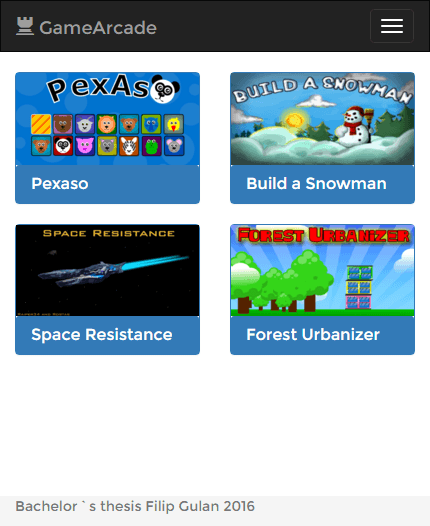
\includegraphics[width=1\textwidth]{fig/ukazka-responzivity.png}
     \end{center}
\end{column}
\end{columns}
\end{frame}

\begin{frame}[fragile]{Implementované riešenie}
    \begin{block}{Aplikačný rámec}
		\begin{itemize}
		\item Sprístupňuje funkcie serveru
        \item Implementácia rozdelená na klientskú časť a serverovú časť
        \item Jednoduchý na použitie 
        \item Dostupná vytvorená dokumentácia
    \end{itemize}
	\end{block}
	\begin{exampleblock}{Príklad použitia}
		\begin{verbatim}
		    this.api = new Api();
		    this.api.initialize('key', function(data, object){
		        if(data['status'] == 0)
		            object.api.store(1, "Some value");
		    }, this)
		\end{verbatim}
	\end{exampleblock}
\end{frame}

\begin{frame}[fragile]{Implementované riešenie}
	\begin{columns}
\begin{column}{0.5\textwidth}

   \begin{block}{Demonštračná hra a testovací skript}
		\begin{itemize}
            \item Demonštračná hra
                \begin{itemize}
                \item Jendoduchá hra PexAso
                \item Implemenotvaná všetka funkcionalita rámca
                \item Phaser
                \end{itemize}
            \item Testovací skript
                \begin{itemize}
                \item Testovanie počas vývoja
                \item Testovanie status položky
                \item Vizualizácia HTML + Javascript
                \end{itemize}
            \end{itemize}
	\end{block}
	
\end{column}
\begin{column}{0.5\textwidth}  %%<--- here
    \begin{center}
     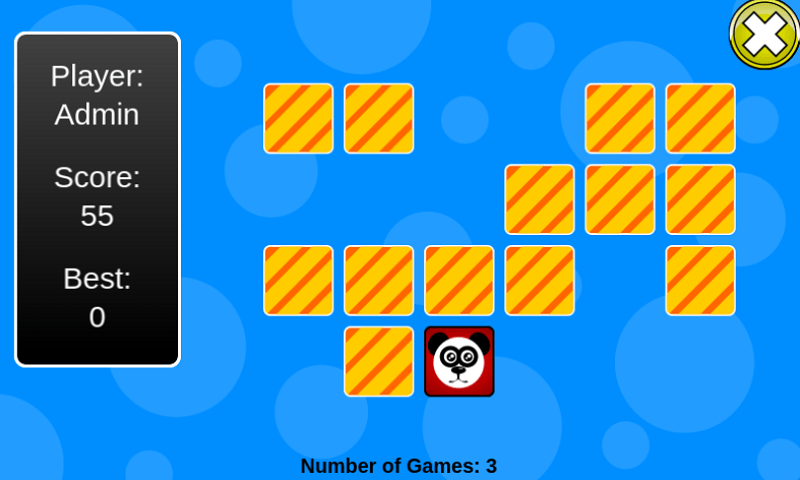
\includegraphics[width=1\textwidth]{fig/ukazka-hra.png}
     \end{center}
\end{column}
\end{columns}
\end{frame}

\begin{frame}[fragile]{Použitie a ďalšie smerovanie projektu}
    \begin{itemize}
        \item Multifunkčný herný portál
        \item Osobné portfólio vývojára
        \item Podpora vývojárov hier
        \item V budúcnosti rozšíriteľné o ďalšie komponenty a moduly aj v rámci webovej platformy aj aplikačného rámca
    \end{itemize}
\end{frame}

\section{Ďakujem za pozornosť}

\begin{frame}[fragile]{Otázky oponenta práce}
    \begin{alertblock}{Popis \textbf{CORS} na straně 23-24 je trochu zmatený. Můžete lépe vysvětlit využití a princip tohoto mechanismu?}
		Kvôli obmedzeniam vychádzajúcich zo \textbf{Same Origin Policy}, kedy nie je možné získavať zdroje, v našom prípade získať odpoveď zo serverovej časti aplikačného rámca,  z inej domény, bolo nutné použitie mechanizmu \textbf{Cross Origin Ressources Sharing}.

        Pre správne použitie \textbf{CORS} musí prehliadač odosielať na server hlavičky \textit{Origin} a server zase musí odpovedať s hlavičkami \textit{Access-Control-Allow-Origin}. 
	\end{alertblock}
\end{frame}

\begin{frame}[fragile]{Otázky oponenta práce}
    \begin{alertblock}{Proč nebylo využito mírně rozšířených tabulek \textit{Storage} a \textit{StorageValue} i pro uložení skóre?}
		Tieto tabuľky neboli použité z dôvodu, že v budúcnosti sa plánuje ďalšie rozšírenie platformy a do týchto tabuliek pribudnú ďalšie nastavenia a terajšia podobnosť sa úplne vytratí. Napríklad pre skóre tabuľky bude možné nastaviť zoradenie hodnôt zostupne/vzostupne a iné. Pre úložiská zase bude pridaná napríklad expirácia uloženej hodnoty… 
	\end{alertblock}
\end{frame}

\end{document}
